%% question-12.tex
%%

%% ==============================
\subsection{Modélisation explicite d'une expression}
\label{sec:question9}
%% ==============================

Le concept d'expression est présenté à l'aide de la figure \ref{fig:expression}. Une \emph{Expression} 

\begin{figure}
	\centering
	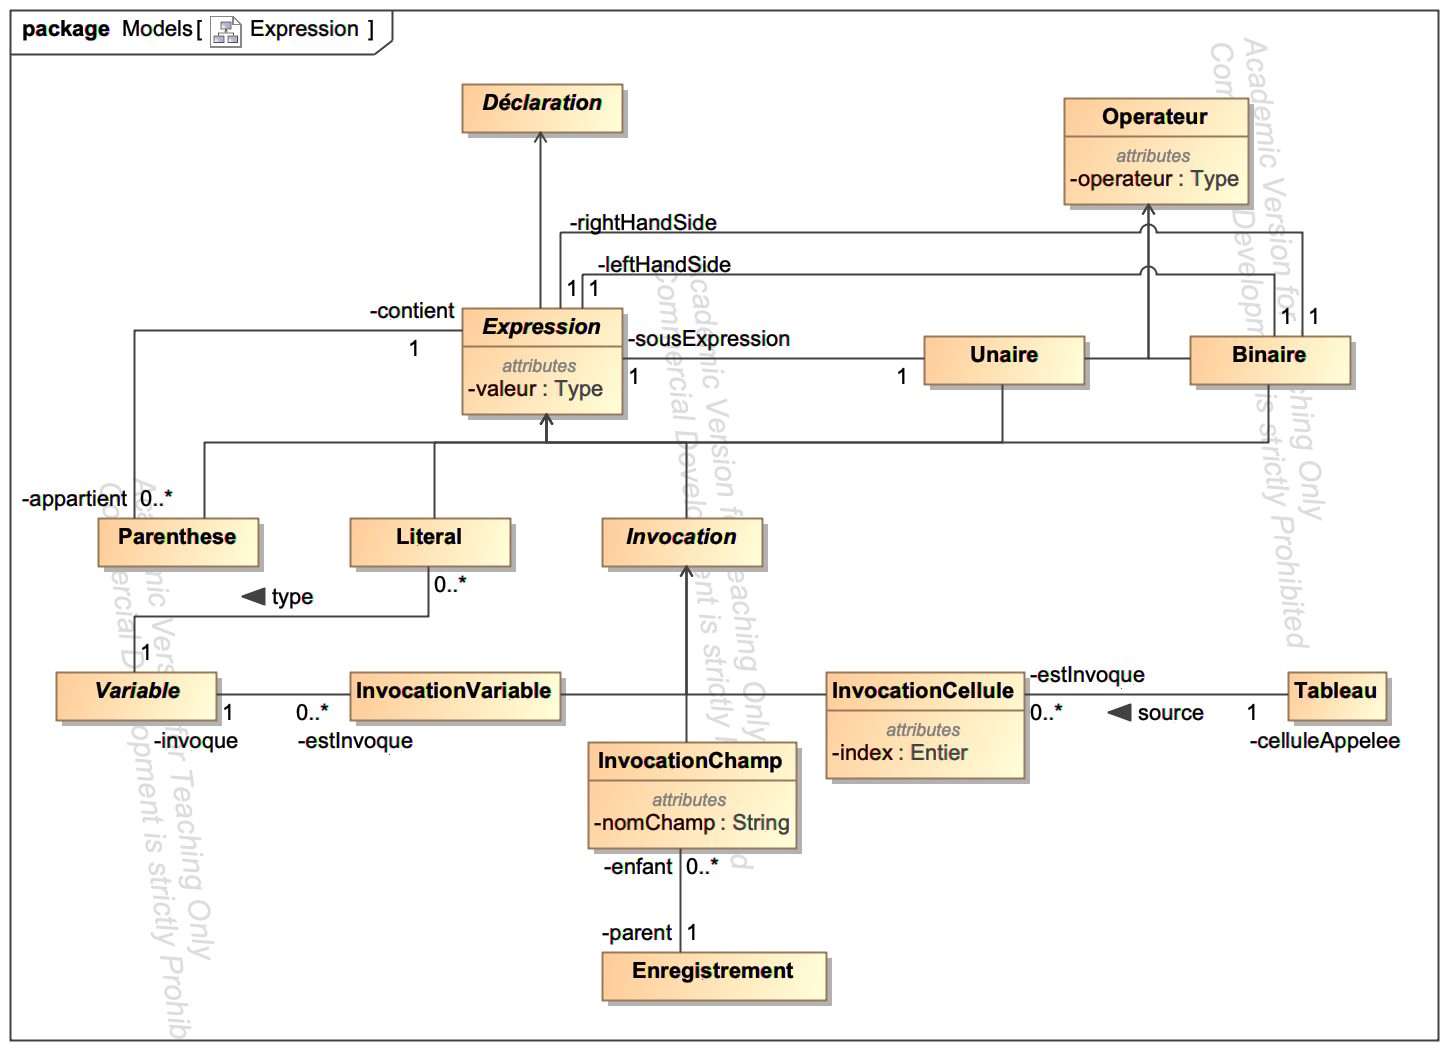
\includegraphics[width=500pt]{assets/class__Expression}
	\caption{Diagramme de classe d'une expression}
	\label{fig:expression}
\end{figure}